\documentclass{standalone}
\usepackage{graphicx}	
\usepackage{amssymb, amsmath}
\usepackage{color}

\usepackage{tikz}
\usetikzlibrary{intersections, backgrounds}

\definecolor{light}{RGB}{220, 188, 188}
\definecolor{mid}{RGB}{185, 124, 124}
\definecolor{dark}{RGB}{143, 39, 39}
\definecolor{highlight}{RGB}{180, 31, 180}
\definecolor{gray10}{gray}{0.1}
\definecolor{gray20}{gray}{0.2}
\definecolor{gray30}{gray}{0.3}
\definecolor{gray40}{gray}{0.4}
\definecolor{gray60}{gray}{0.6}
\definecolor{gray70}{gray}{0.7}
\definecolor{gray80}{gray}{0.8}
\definecolor{gray90}{gray}{0.9}
\definecolor{gray95}{gray}{0.95}

\newcommand*{\offset}{0.025}

\begin{document}

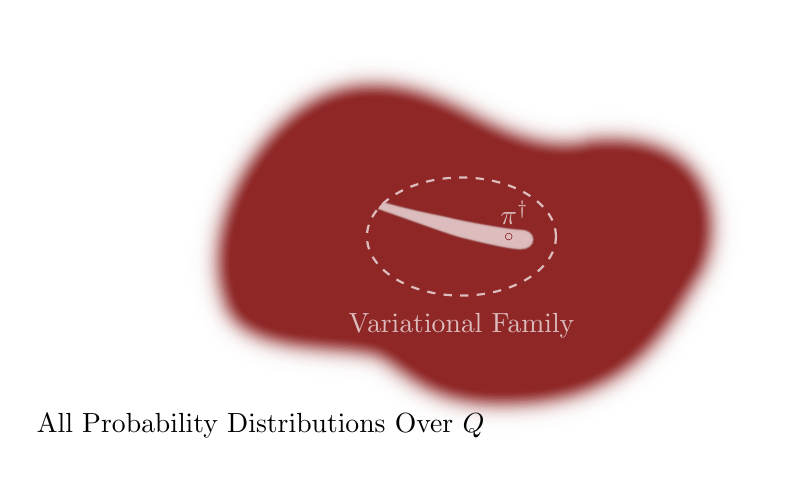
\begin{tikzpicture}[scale=0.15, thick]               
 \pgfmathsetmacro{\dx}{0}
 
 \foreach \i in {1, 0.975, ..., 0} {
   \pgfmathsetmacro{\prop}{100 * exp(-10.0 * \i * \i)};
   \colorlet{custom}{dark!\prop!white};
   \draw[line width={40 * \i}, color=custom] 
     (\dx + -20, -2)
    .. controls (\dx + -22, 4) and (\dx + -17, 12) .. (\dx + -12, 14)  
    .. controls (\dx + -7, 16) and (\dx + -2, 13) .. (\dx + 0, 12)
    .. controls (\dx + 2, 11) and (\dx + 6, 9) .. (\dx + 10, 10)
    .. controls (\dx + 20, 11) and (\dx + 20, 3) .. (\dx + 18, 0)
    .. controls (\dx + 15.5, -4) and (\dx + 13, -9.5) .. (\dx + 4, -10)
    .. controls (\dx + -4, -10.5) and (\dx + -5, -7) .. (\dx + -8, -6)
    .. controls (\dx + -11, -5) and (\dx + -19, -6) .. (\dx + -20, -2);
  }
  
  \fill [dark] (\dx + -20, -2)
    .. controls (\dx + -22, 4) and (\dx + -17, 12) .. (\dx + -12, 14)  
    .. controls (\dx + -7, 16) and (\dx + -2, 13) .. (\dx + 0, 12)
    .. controls (\dx + 2, 11) and (\dx + 6, 9) .. (\dx + 10, 10)
    .. controls (\dx + 20, 11) and (\dx + 20, 3) .. (\dx + 18, 0)
    .. controls (\dx + 15.5, -4) and (\dx + 13, -9.5) .. (\dx + 4, -10)
    .. controls (\dx + -4, -10.5) and (\dx + -5, -7) .. (\dx + -8, -6)
    .. controls (\dx + -11, -5) and (\dx + -19, -6) .. (\dx + -20, -2);
    
  \node [] at (\dx + -18, -13) { All Probability Distributions Over $Q$ };
  
  \begin{scope}
    \clip (\dx + -1, 3) circle (8 and 5);

    \foreach \i in {0, 0.01,..., 1} {
    \draw[opacity={exp(-8 * \i * \i)}, light, line width={5 * \i}] (\dx + -9, 6) 
      .. controls (\dx + -6, 5) and (\dx + -3, 4.5) .. (\dx + -2, 4.25)
      .. controls (\dx + -1, 4) and (\dx + 3, 3.25) .. (\dx + 4, 3.25)
      .. controls (\dx + 5, 3.25) and (\dx + 5, 2.25) .. (\dx + 4, 2.25) 
      .. controls (\dx + 3, 2.25) and (\dx + -0, 3) .. (\dx + -1, 3.25)
      .. controls (\dx + -2, 3.5) and (\dx + -6, 5) .. (\dx + -9, 6);
    }
  
    \fill[light] (\dx + -9, 6) 
      .. controls (\dx + -6, 5) and (\dx + -3, 4.5) .. (\dx + -2, 4.25)
      .. controls (\dx + -1, 4) and (\dx + 3, 3.25) .. (\dx + 4, 3.25)
      .. controls (\dx + 5, 3.25) and (\dx + 5, 2.25) .. (\dx + 4, 2.25) 
      .. controls (\dx + 3, 2.25) and (\dx + -0, 3) .. (\dx + -1, 3.25)
      .. controls (\dx + -2, 3.5) and (\dx + -6, 5) .. (\dx + -9, 6);
  \end{scope};
      
  \draw[color=light, dashed] (\dx + -1, 3) circle (8 and 5);

  \node[light] at (\dx + -1, -4.5) {Variational Family};
  
  \fill[dark] (\dx + 3, 3) circle (\dx + 9pt); 
  \fill[light] (\dx + 3, 3) circle (\dx + 7pt); 
  \node[light] at (\dx + 3.5, 5) {$\pi^{\dagger}$};
 \end{tikzpicture}

\end{document}   